\documentclass[amssymb, aps,nofootinbib, superscriptaddress, notitlepage]{revtex4}
\usepackage{nccmath}
\usepackage[mathscr]{eucal}
\usepackage[dvips]{graphicx}
\usepackage{amsfonts,amssymb,amsmath,bbm}
\usepackage[all]{xy}  % xy diagrams
\usepackage{tikz}  
\usepackage{xcolor}
\usepackage[T1]{fontenc} % if needed
\usepackage{slashed}
\usepackage{feynmp}
\usepackage{epsfig}
\usepackage{tikz}
\usepackage{enumerate}
 \usepackage{algorithm}
 \usepackage{algpseudocode}
\begin{document}

\title{Report for Assignment 2 of Foundations of High Performance Computing 2021/2022}
\date{\today}


\author{Marco Celoria}
\email{celoria.marco@gmail.com}
\affiliation{Master in High Performance Computing SISSA/ICTP}
%
%\begin{abstract}
%Report for Assignment 1 of Foundations of High Performance Computing 2021/2022
%\end{abstract}
\maketitle
\section{Introduction}
For the second assignment of Foundations of High Performance Computing we have to implement a parallel kd-tree, namely  a binary tree in which every node is associated to a $k$-dimensional point. Specifically, we have considered the  case $k=2$, but what follows may be straightforwardly generalized for arbitrary $k$.
\\
The idea is that given a set of points (and particularly we assume a homogeneously distribution of points) in a 2-dimensional plane (for example the region $[0,1]\times [0,1]$), we identify the non-leaf (or splitting) nodes as the ones corresponding to a point (the splitting point) dividing the plane into two parts.
Moreover, each node is associated to a direction (the splitting direction), say $i$-coordinate with $i=x,y$, and has two children nodes (left node and right node).
\\
We define the left points  as the ones with $i$-coordinate smaller than the $i$-coordinate of the splitting point, the right points are those with larger $i$-coordinate.  The left (right) points will then be assigned to the left (right) sub-tree, i.e. the branch generated by the left (right) child node. 
\\
 Finally, when only one point remains at the end of the tree, we assign this point to the leaf node.

We have considered two parallel codes both written in C, one using  OpenMP and the other  MPI.
The strategy is similar for the two cases: start with a root node, divide the points among two workers $L$ and $R$, which will create simultaneously (in parallel) the left and right sub-trees.
If there are free workers, $L$ and $R$ can eventually divide their tasks  with other two and so on, until  all the available workers are busy.
In this final condition,  each worker has to serially build its own sub-tree till the leafs.

\section{Kd-tree: Shared Memory algorithm}

First of all, let us present the serial/shared memory algorithm we have implemented.
\\
Given the node $\mathcal{T}$, the associated set of points  $X_\mathcal{T}$ and  the previous splitting direction $p_{\mathcal{T}_{-}}$, the serial/shared-memory algorithm is described in Algorithm \ref{alg:Serial/SharedKdTree}, where $\tilde{x}_{p_{\mathcal{T}}}$ is the splitting point associated to the node $\mathcal{T}$ and $p_{\mathcal{T}}$ is the current splitting direction.
Moreover,  $\{\dots\}$ indicates the OpenMP parallelization.


\begin{algorithm}
\caption{Serial/Shared KdTree build function}\label{alg:Serial/SharedKdTree}
\begin{algorithmic}
\State  $\textsc{Serial/SharedKdTree}(\mathcal{T},X_\mathcal{T},p_{\mathcal{T}_{-}})$
\State $N= |X_\mathcal{T}| $
\If{$ l_{\mathcal{T}} == \textsf{maxLevel} \ || \ N < \textsf{minNumofPoints} $} 
 \State $\text{store } X_\mathcal{T} \text{ in }\mathcal{T}$
  \State $\text{return}$
\EndIf
 \State $p_{\mathcal{T}}= \textsc{SplitDirection}(p_{\mathcal{T}_{-}}) $
  \State $\tilde{x}_{p_{\mathcal{T}}} = \textsc{QuickSelect}(X_\mathcal{T},\frac{N}{2},p_\mathcal{T})$
   \State{$X_l: x^i \in X_\mathcal{T}  \ | \ x^i_{p_{\mathcal{T}}}  < \tilde{x}_{p_{\mathcal{T}}} $}
    \State{$X_r: x^i \in X_\mathcal{T}  \ | \ x^i_{p_{\mathcal{T}}} > \tilde{x}_{p_{\mathcal{T}}} $}
     \State $\{\text{Task}\}:\ \textsc{Serial/SharedKdTree}(\text{LeftChild}(\mathcal{T}),X_l, p_{\mathcal{T}})$
       \State $\{\text{Task}\}:\ \textsc{Serial/SharedKdTree}(\text{RightChild}(\mathcal{T}),X_r, p_{\mathcal{T}})$
\end{algorithmic}
\end{algorithm}
 
The function $\textsc{SplitDirection}$ chooses the splitting direction  round-robin, see Algorithm \ref{alg:SplitDirection}, with $k=2$.
\\
 $\textsc{QuickSelect}$ is a standard selection algorithm to find the $n$-th smallest element in an unordered list. 
To find the median, we have considered $n=\frac{N}{2}$.  
Note that $\textsc{QuickSelect}$  also partially sorts the data.


\begin{algorithm}
\caption{Find split direction function}\label{alg:SplitDirection}
\begin{algorithmic}
\State  $\textsc{SplitDirection}(p_{\mathcal{T}_{-}}) $
\State $\text{return} \ (p_{\mathcal{T}_{-}}+ 1) \% k$
\end{algorithmic}
\end{algorithm}


\section{Kd-tree: distributed MPI algorithm}
For the MPI code, we choose to implement a distributed memory kd-tree, inspired by \cite{xiao2016parallel}.
\\
We have implemented two versions, the first is very simple but imprecise/approximated and is described in Algorithm \ref{alg:A2A},  where $C_\mathcal{T}$ indicates the communicator associated to the node $\mathcal{T}$.

\begin{algorithm}
\caption{Distributed KdTree build function based on AllToAll MPI routine}\label{alg:A2A}
\begin{algorithmic}
\State  $\textsc{DistributedKdTreeA2A}(\mathcal{T},X_\mathcal{T},p_{\mathcal{T}_{-}},C_\mathcal{T})$
\State $N= |X_\mathcal{T}| $
\If{$|C_\mathcal{T}|==1  \ || \ \ell_\mathcal{T}==\textsf{maxLevel} \ || \ N < \textsf{minNumofPoints}$} 
 \State $\textsc{Serial/SharedKdTree}(\mathcal{T}, X_\mathcal{T},p_{\mathcal{T}_{-}})$
  \State $\text{return}$
  \EndIf
 \State $p_{\mathcal{T}}= \textsc{SplitDirection}(p_{\mathcal{T}_{-}})$
  \State $\tilde{x}_{p} = \textsc{QuickSelect}(X_\mathcal{T}, \frac{N}{2},p_{\mathcal{T}})$
   \State $X^{new} = \textsc{PointRepartition}(X_\mathcal{T}, C_\mathcal{T}) $
    \State $C^{new} = \textsc{CommSplit}(C_\mathcal{T})$
     \State $\textsc{DistributedKdTreeA2A}(\text{Kid}(\mathcal{T}),X^{new},p_{\mathcal{T}},C^{new})$
\end{algorithmic}
\end{algorithm}
 
The function $\textsc{PointRepartition}$ is given by Algorithm \ref{alg:A2A_PointRepartition}.

\begin{algorithm}
\caption{PointRepartition function for AllToAll KdTree}\label{alg:A2A_PointRepartition}
\begin{algorithmic}
\State  $\textsc{PointRepartition}(X_\mathcal{T}, C_\mathcal{T}) $
\State $\text{return} \ \textsc{AllToAll}(X_\mathcal{T}, C_\mathcal{T})$
\end{algorithmic}
\end{algorithm}

One difference with respect to \cite{xiao2016parallel} is how we find the splitting dimension as we use the same strategy as before, i.e.  round-robin. 
Another difference is that we have simplified the $\textsc{PointRepartition}$ function, specifically we have used a simple $\textsf{MPI\_Alltoall}$ while in \cite{xiao2016parallel} a complicated function based on $\textsf{MPI\_Alltoallv}$ is presented. 
\\
As we will explain later, while the implementation based on $\textsf{MPI\_Alltoallv}$ results in the correct kd-tree, our simple implementation, based on $\textsf{MPI\_Alltoall}$, returns only an approximated kd-tree.
\\
For this reason, we have implemented  another algorithm, proposed again in \cite{xiao2016parallel}, that is more accurate but also more complicated.
\\
Such algorithm is described by Algorithm \ref{alg:P2P}, where  $N^{tot}_{C}$ is the total number of points in the communicator, $\textsc{PointRepartition}$ function  is given by  Algorithm \ref{alg:P2P_PointRepartition} and $\textsc{ParSelect}$ is described in   Algorithm \ref{alg:P2P_ParSelect}.

\begin{algorithm}
\caption{Distributed KdTree build function for Pointwise exchange KdTree}\label{alg:P2P}
\begin{algorithmic}
\State  $\textsc{DistributedKdTreeP2P}(\mathcal{T},X_\mathcal{T},p_{\mathcal{T}_{-}},C_\mathcal{T})$
\State $N=|X_\mathcal{T}| $
\State $N^{tot}_{C}=\textsc{Allreduce}(N)$
\If{$|C_\mathcal{T}|==1  \ || \ \ell_\mathcal{T}==\textsf{maxLevel} \ || \ N < \textsf{minNumofPoints}$} 
    \State $\textsc{Serial/SharedKdTree}(\mathcal{T}, X_\mathcal{T},p_{\mathcal{T}_{-}})$
    \State $\text{return}$
\EndIf 
     \State $p_{\mathcal{T}}= \textsc{SplitDirection}(p_{\mathcal{T}_{-}}) $
        \State $m_\mathcal{T} = \textsc{ParSelect}(X_\mathcal{T},N^{tot}_{C}/2,p_{\mathcal{T}}, C_\mathcal{T})$
        \For {$x_i\in X_\mathcal{T}$}
        \If{$x^i_{p_{\mathcal{T}}} < m_\mathcal{T}$}
        \State $\text{assign } x_i \text{ to }  X_l$
  \Else
        \State $\text{assign } x_i \text{ to }  X_r$
        \EndIf
        \EndFor
        \State $X^{new} = \textsc{PointRepartition}(X_l,X_r, C_\mathcal{T})$
        \State $C^{new} = \textsc{CommSplit}(C_\mathcal{T})$
        \State $\textsc{DistributedKdTreeP2P}(\text{Kid}(\mathcal{T}),X^{new},p_{\mathcal{T}},C^{new})$
\end{algorithmic}
\end{algorithm}

\begin{algorithm}
\caption{PointRepartition function for Pointwise exchange KdTree}\label{alg:P2P_PointRepartition}
\begin{algorithmic}
\State $\textsc{PointRepartition}(X_l,X_r, C_\mathcal{T})$
\State $r = \text{rank}(C_\mathcal{T})$
\State $s = \text{size}(C_\mathcal{T})$
\If{$r< s/2$} 
    \State $\text{Send } X_r \text{ to rank }  (s-r)$
    \State $\text{Receive }  X'_l \text{ from rank }  (s-r)$
\Else
    \State $\text{Send } X_l \text{ to rank }  (s-r)$
      \State $\text{Receive } X'_r \text{ from rank } (s-r)$   
\EndIf 
\end{algorithmic}
\end{algorithm}

\begin{algorithm}
\caption{ParSelect function for Pointwise exchange KdTree}\label{alg:P2P_ParSelect}
\begin{algorithmic}
\State {$\textsc{ParSelect}(arr, k, p_{\mathcal{T}}, C_\mathcal{T})$}
\State{$N = \textsc{AllReduce}(arr.size())$}
 \State{$m_{\mathcal{T}} = \textsc{GlobalMean}(arr, p_{\mathcal{T}},C_\mathcal{T})$}
  \State {$arr\_less=[]$} 
  \State {$arr\_great=[]$} 
  \For {$\text{each point } i  \text{ in input array } arr$}
  \If{$arr[i]_{\text{projected on direction }p_{\mathcal{T}}} > m_{\mathcal{T}} $}
  \State{$arr\_less.insert( arr[i] )$}
  \Else
  \State{$arr\_great.insert( arr[i] )$}
  \EndIf
  \EndFor
  \State {$N_l = \textsc{AllReduce}(arr\_less.size())$}
    \State {$N_g = \textsc{AllReduce}(arr\_great.size())$}
  \If{$N==1 \ || \ N_l==k \ || \ N_l==N \ | \ N_g==N$}
  \State{$\text{return } m_{\mathcal{T}} $}
  \ElsIf{$N_l > k$}
\State  {$\textsc{ParSelect}(arr\_less, k,p_{\mathcal{T}}, C_\mathcal{T})$}
  \Else
  \State {$\textsc{ParSelect}(arr\_great, k - N_l,p_{\mathcal{T}}, C_\mathcal{T})$}
\EndIf 
\end{algorithmic}
\end{algorithm}

This is the general idea for our distributed algorithm, however there are still different choices we have to do that will be discussed in details  in the next Section.

\section{Implementation}
\subsection{General consideration}

Let us start our discussion concerning the implementations by mentioning some general considerations.
Actually, many choices are possible. 
\\
First of all, concerning the splitting direction, given our assumptions we opted for a simple round-robin approach, with the advantage of being an $\mathcal{O}(1)$ operation.
\\
Other possible choices include, see for instance \cite{xiao2016parallel}
\begin{itemize}
\item[$\dagger$] selecting a coordinate axis at random (that is another possible $\mathcal{O}(1)$ operation);
\item[$\ddagger$] choosing the coordinate with the largest variance considering all points within a node;
\item[$\ddagger$] choosing the direction where the points are furthest apart.
\end{itemize}
These latter two possibilities require scanning the data set and might be very useful if data are not homogeneously distributed or are distributed in a very narrow stripe.
 However, we decided to keep this operation as simple/fast as possible, and round robin is a valid option for data homogeneously distributed within a square.
\\
Another issue is the choice of the splitting point, where we opted for the median. To find the median, we use a select algorithm to find the $N/2$-th smallest element in an array.
For instance, the standard Quickselect algorithm, used in the OpenMP code as well as in the serial part of the MPI code,  has  average complexity of $\mathcal{O}(N)$, with a worst case of $\mathcal{O}(N^2)$.
For the distributed memory algorithm (parallel part of the MPI code) we  look for the global median with a similar selection algorithm, with complexity of the order of $\mathcal{O}(t_c \log P \log N + N/P)$, for details see  \cite{xiao2016parallel}.

\subsection{Shared OpenMP kd-tree}
Our main focus is the distributed memory kd-tree, as the serial kd-tree is well known and our implementation of the shared memory (OpenMP) kd-tree is directly based on the serial algorithm.
Parallelization is achieved by opening a parallel region, spawning threads that will execute their own tasks  in an effective and parallel way.
\\
Referring to the Introduction, here  the workers/threads perform the OpenMP tasks, building the tree from the data available on the memory of a single node (data-points are shared).  As long as threads are available, at each level in the tree, two new tasks are created, associated to the left and right sub-tree. 
\\
Finally, to avoid possible overhead associated to an uncontrolled creation of tasks, we regulate task parallelism according to the number of threads available (or equivalently the level depth).
In Figure \ref{serialTree}, starting with 64 random points we show the resulting tree obtained with the serial and the OpenMP code (the resulting tree is the same for both codes). 

\begin{figure}
  \centering
      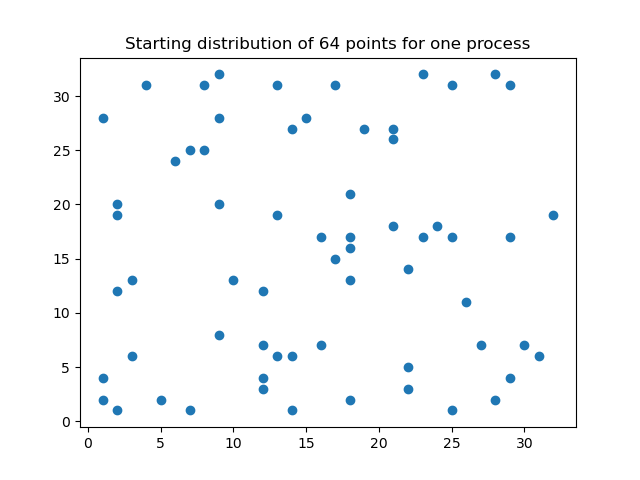
\includegraphics[width=0.49\textwidth]{img/Starting_64_shared.png}
      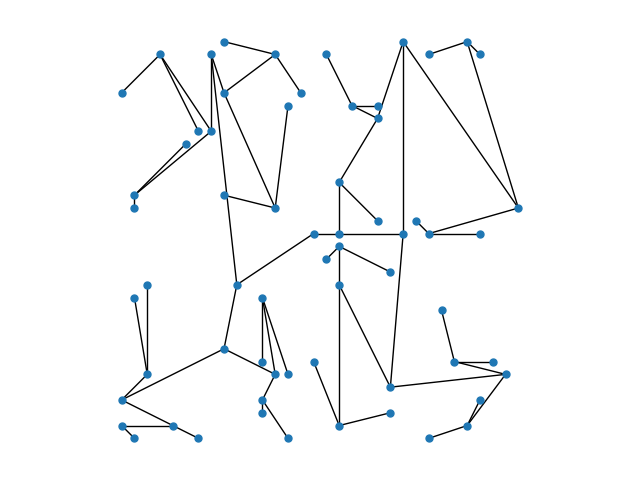
\includegraphics[width=0.49\textwidth]{img/serial64.png}
     % 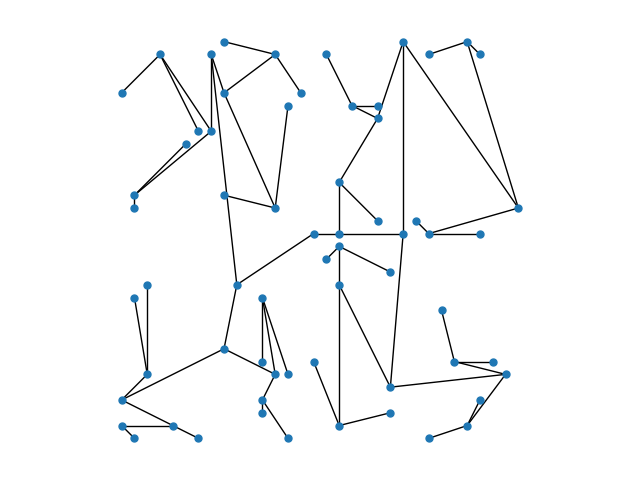
\includegraphics[width=0.49\textwidth]{img/openmp64.png}
 \caption{From the original 64 data points (Left), we can see the final tree produced by the serial and the OpenMP code  (Right) produced on Login node on ORFEO cluster (with 20 threads for OpenMP). The results for the serial and OpenMP codes are equivalent, and we show only one to avoid redundancies.}
\label{serialTree}
\end{figure}



\subsection{Distributed MPI kd-tree}


The main difference between OpenMP and MPI is that 
\begin{itemize}
\item OpenMP $\Longrightarrow$ Shared memory
\item MPI $\Longrightarrow$ Distributed memory
\end{itemize}
This means that for MPI two possible choices are available.
\begin{enumerate}
\item[a)] all processes work on the same $N_{tot}$ (total) points.
\\
 In this case, the maximum size of the kd-tree is limited by the memory of a single node.
\item[b)] each process works on $N_{tot}/P$ points where $P$ is the number of processes. 
\\
In this case, the maximum size of the kd-tree is bounded by the number of nodes available.
\end{enumerate}
We have opted for the second option, namely a distributed kd-tree, and for this reason the final structure of the kd-tree is different from the shared-memory one.
\\
In this distributed approach, the workers of the Introduction are the MPI processes in communicators, exchanging points among them-self to collectively build the  kd-tree. 
\\
The idea is that at each level/iteration the MPI communicator is  splitted in two, the processes with rank $l<\frac{\text{s}}{2}$ (where $s$ is the size of the communicator) create the left communicator $C_l$, while the others $r'$ constitute the right communicator $C_r$. 
Processes belonging to the  left communicator have to send their right points (with respect to the global median)  to the right processes and receive back the  left points   \footnote{Eventually, they might want to redistribute the points among the corresponding  $C_l$ (or $C_r$)  sub-communicator, in such a way that at the end, every processes have the same number of points. However, we have not implemented such re-balancing since it should not be need as we assume that data are homogeneously distributed.}.  
Finally,  we recursively build the distributed kd-tree with a unique kid (a parallel kid) as long as the size of the communicator is more than one. When there is only one process in the communicator, we proceed with the serial algorithm.

\begin{figure}
  \centering
      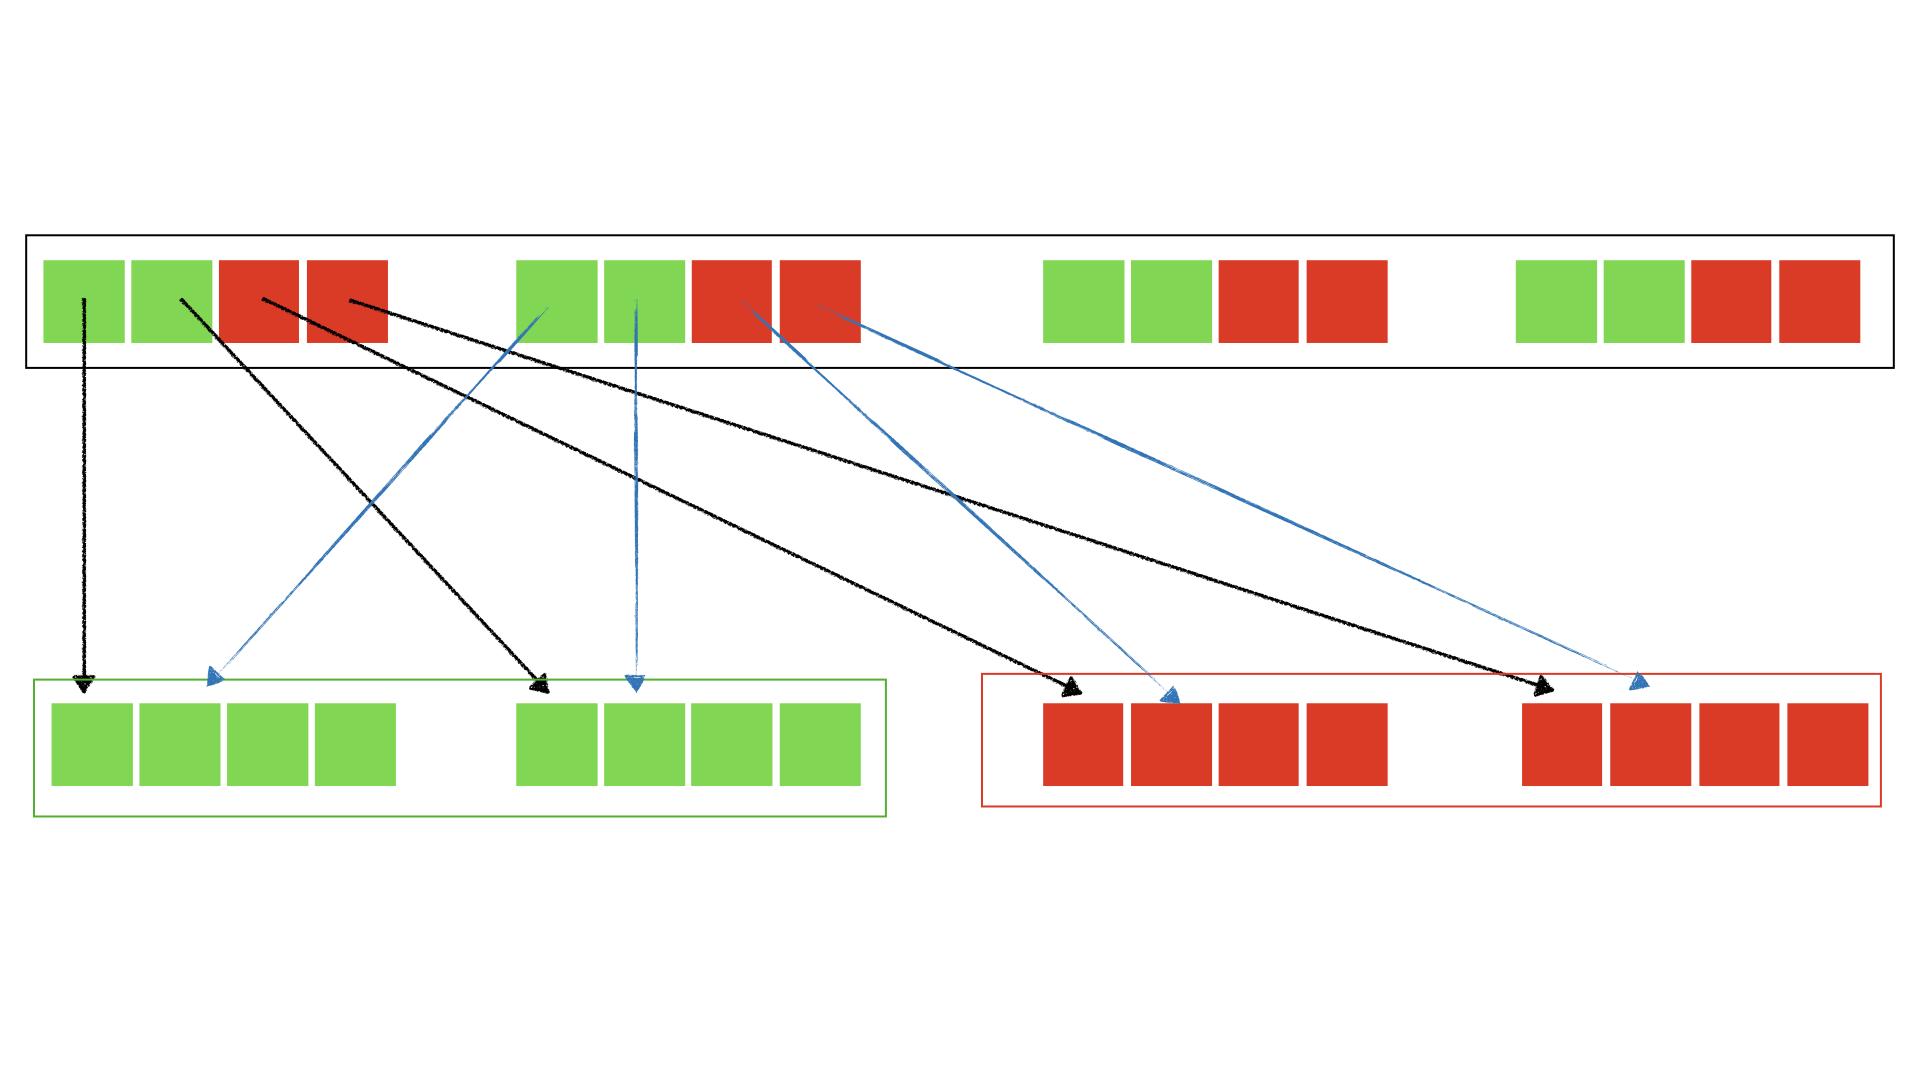
\includegraphics[width=0.49\textwidth]{img/all2all.png}
 \caption{Schematic representation of the AllToAll communication, for simplicity some arrows are missing in the Figure.
 Since data are homogeneously distributed it is reasonable to approximate the global median with the local median.
Consider four processes in the communicator, each with half points (green blocks) smaller than the local splitting point (left points are sorted because of the Quickselect algorithm) and half greater (red blocks). After redistributing the points by means of the AllToAll communications, all left points will belong the the first two processes and the right points to the last two processes. Finally, we split the original communicator in left  $C_l$ and  right communicator $C_r$.}
\label{all2all}
\end{figure}
\subsubsection{Simple AllToAll}
We started from a simple implementation, where, under the  hypothesis that points are homogeneously distributed,   the global median, on average, will be approximated by the local median. As a consequence, each process  (with say $N$ points) will statistically (but not exactly) have $\frac{N}{2}$ points smaller than the global median and $\frac{N}{2}$ greater. Under this approximation, we can keep the number of points per process constant and greatly simplify the coding part as points can be redistributed among the processes by means of a simple $\textsf{MPI\_Alltoall}$ routine, as depicted in Figure \ref{all2all}.
Unfortunately,  the resulting kd-tree is not exact: for instance it might happen that a small fraction of points greater than the global median will be assigned to the left communicator (left sub-tree) and viceversa. This misplaced fraction is clearly larger for smaller dataset, see Figure \ref{Comparison_128} and \ref{Comparison_1024}. 
In Figure \ref{A2A}, we start from 64 random points distributed among 4 processes and we show the resulting kd-tree based on the A2A algorithm.
\begin{figure}
  \centering
      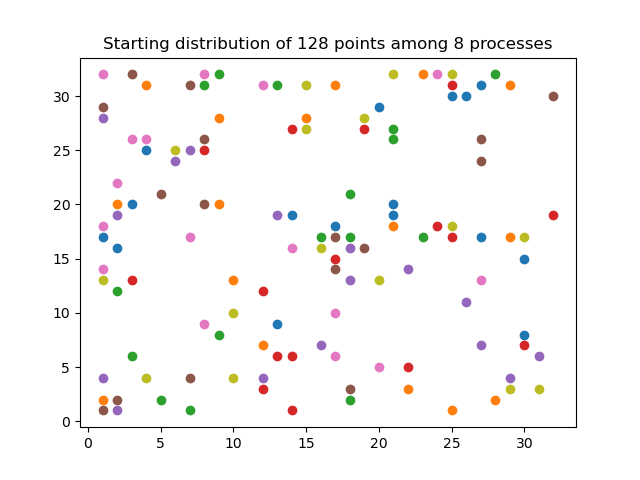
\includegraphics[width=0.32\textwidth]{img/Starting_128.png}
      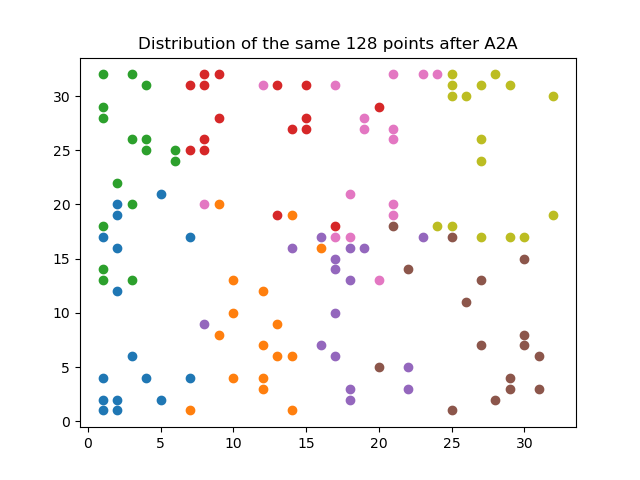
\includegraphics[width=0.32\textwidth]{img/A2A_128.png}
      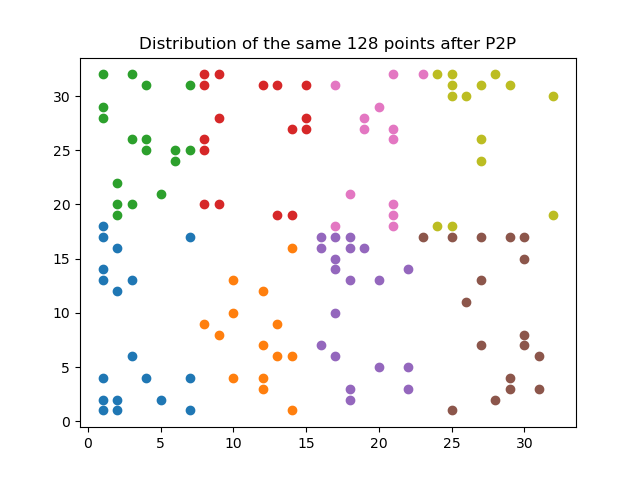
\includegraphics[width=0.32\textwidth]{img/P2P_128.png}
 \caption{Starting from a given distribution of 128 random points among 8 processes (Left), we compare the distribution of points after the parallel part has completed (corresponding to the distribution of points at the beginning of the serial part) for the AllToAll (A2A - Center) and the Pointwise communication (P2P - Right) implementation. As we can see, the clustering for the simple A2A implementation is just approximated and not definite, meaning that some points are misplaced. Conversely, the P2P implementation returns the correct result.}
\label{Comparison_128}
\end{figure}

\begin{figure}
  \centering
  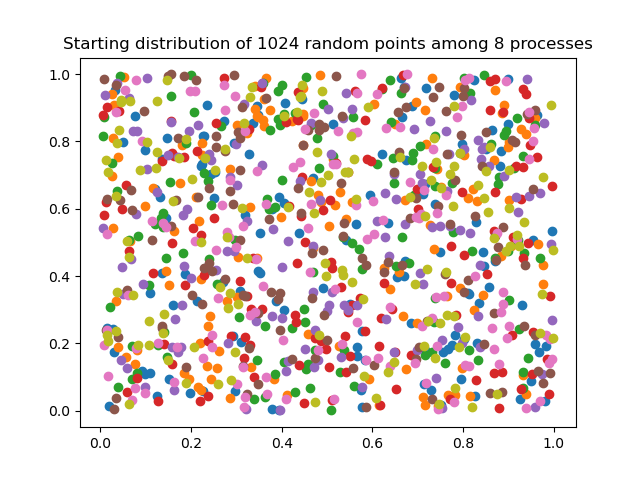
\includegraphics[width=0.32\textwidth]{img/Starting_1024.png}
      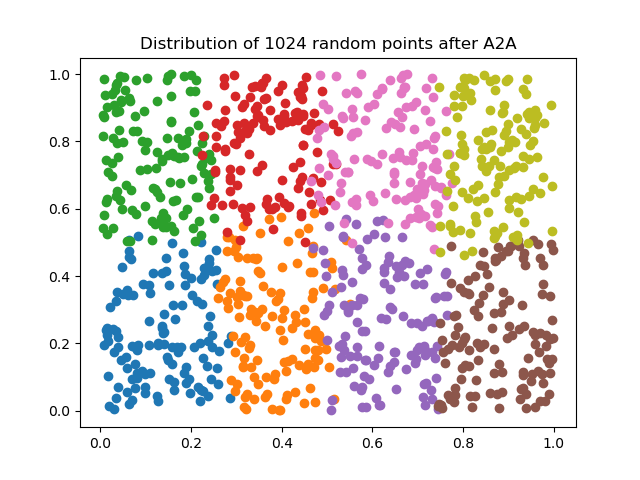
\includegraphics[width=0.32\textwidth]{img/A2A_1024.png}
      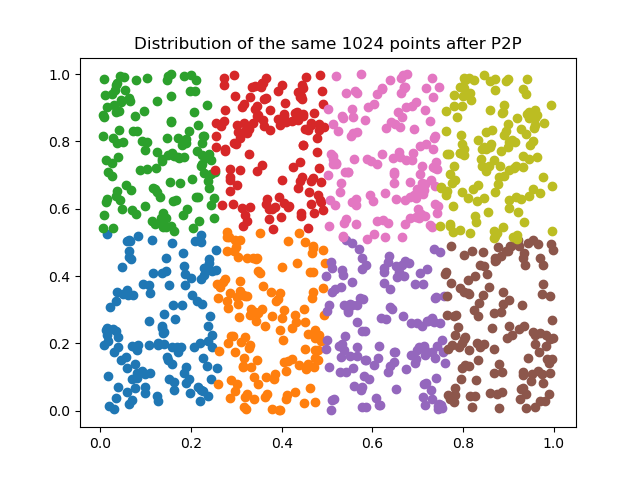
\includegraphics[width=0.32\textwidth]{img/P2P_1024.png}
 \caption{By considering more points, here 1024 random points originally distributed among 8 processes, we can see that the AllToAll approximation is more justified, the clustering is similar, meaning that statistically all the points are correctly redistributed among the processes. Again,  for the Pointwise exchange implementation, the result is exact.}
\label{Comparison_1024}
\end{figure}


\begin{figure}
  \centering
      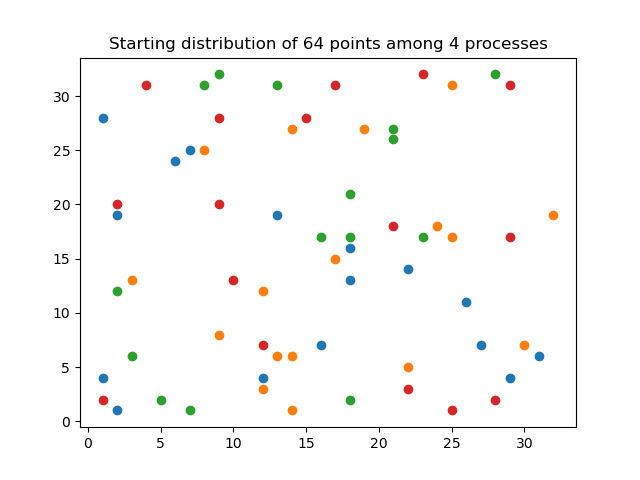
\includegraphics[width=0.45\textwidth]{img/Starting_64.png}
            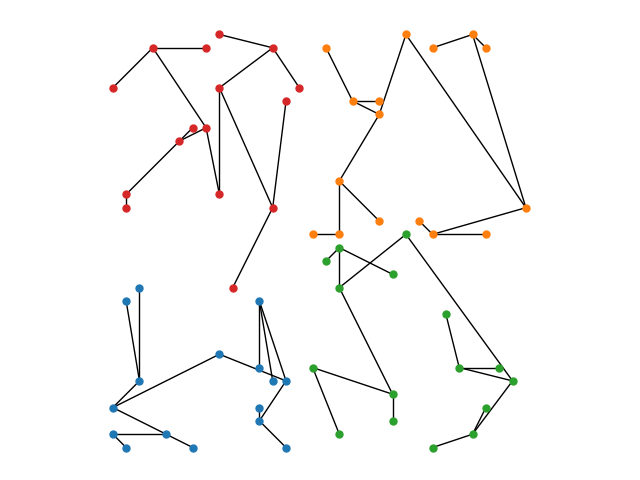
\includegraphics[width=0.45\textwidth]{img/mpiA2A.png}
 \caption{Simple AllToAll algorithm. 
 The original 64 random points are shown on the Left. 
On the Right we show the final kd-tree obtained with the (actually  \textbf{moving})  A2A algorithm.}
\label{A2A}
\end{figure}


\begin{figure}
  \centering
      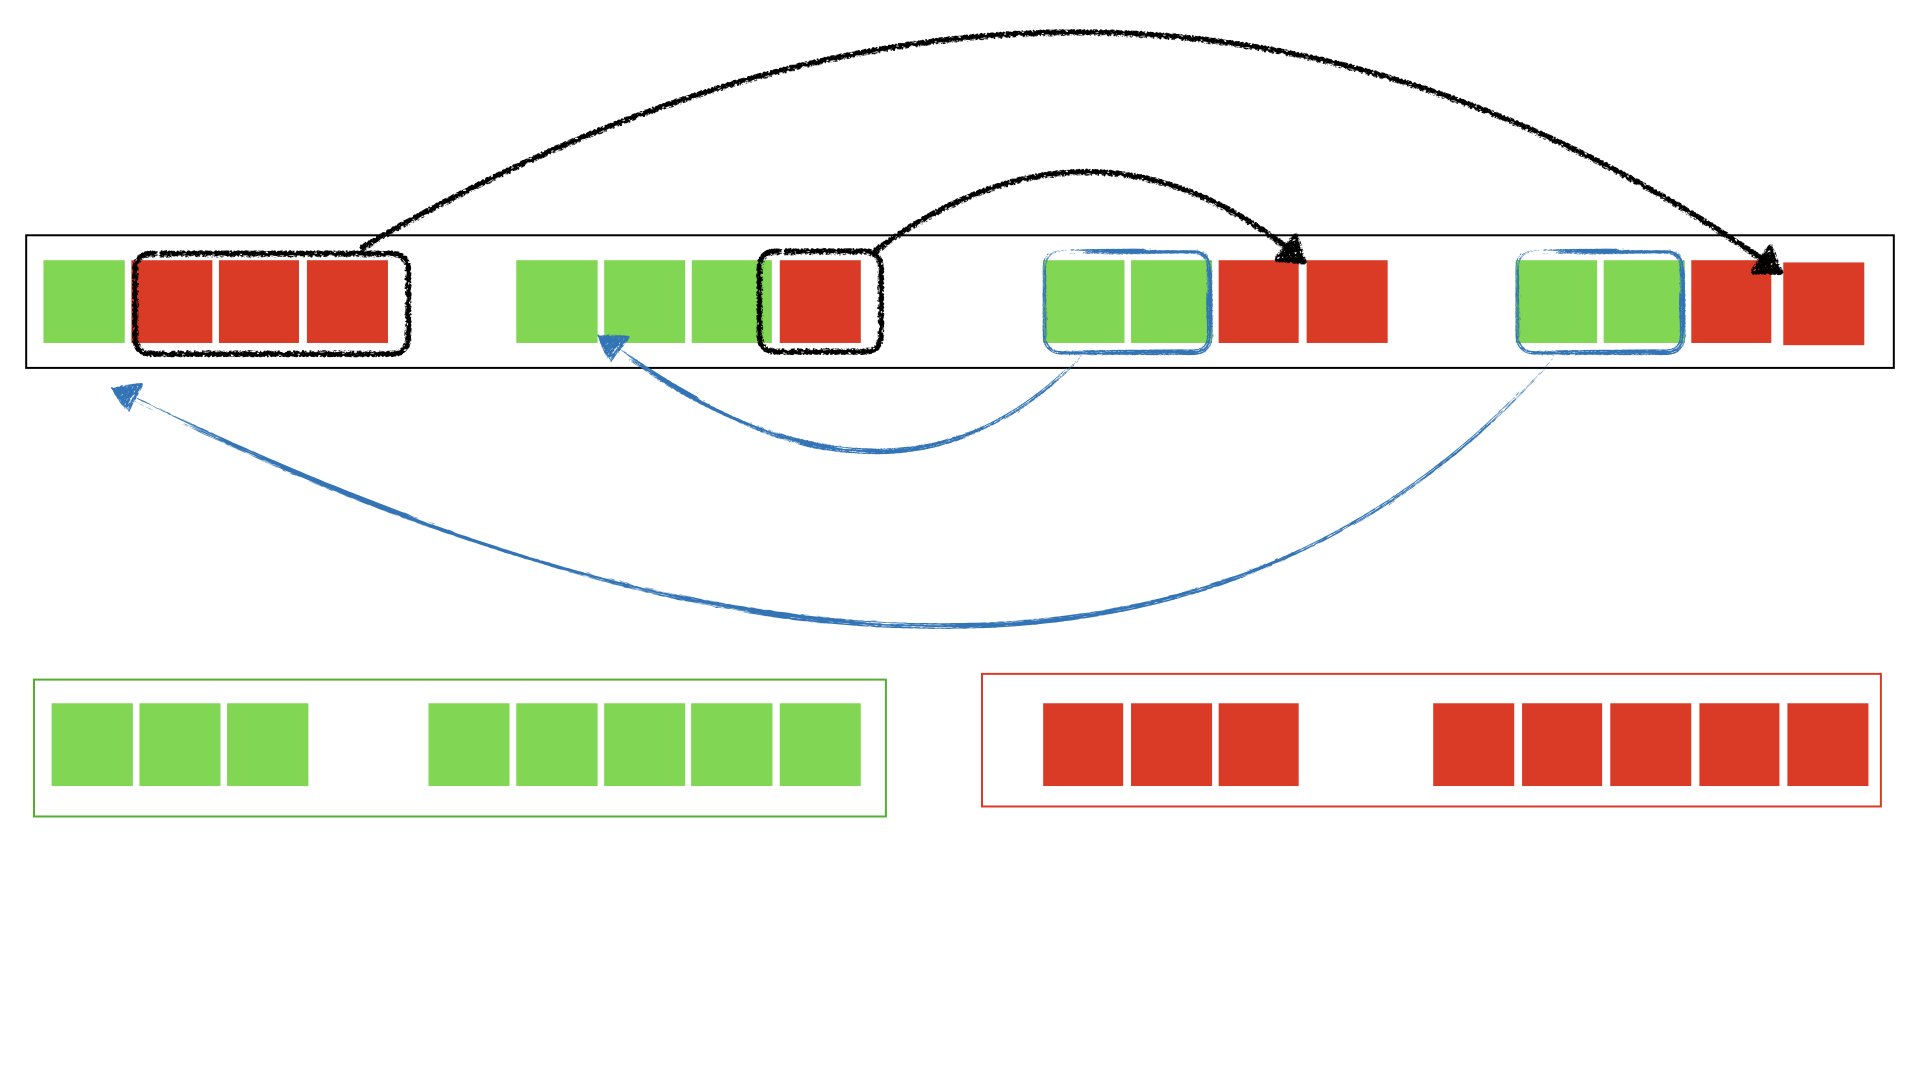
\includegraphics[width=0.49\textwidth]{img/point2point.png}
 \caption{Schematic representation of the Pointwise communication. After looking for the global median $m_\mathcal{T}$, each of the four processes in the original communicator organize their points in left and right arrays with respect to $m_\mathcal{T}$. Then  we perform pointwise communication so that, at the end, all left points are on rank 0 and rank 1, while right points on rank 2 and rank 3.  Finally, we split the communicator in left and right communicators.
The final load might not be balanced and one can redistribute the points among the left  and right communicator. However, we have not implemented such re-balancing as, due to the homogeneous hypothesis, such unbalance is expected to be small.}
\label{point2point}
\end{figure}



\subsubsection{Pointwise exchange}
In order to build an accurate kd-tree we have  implemented a different algorithm based on pointwise data exchange.
The idea is that (see Figure \ref{point2point}), after finding the  splitting direction (say $p_\mathcal{T}$) with a simple round-robin approach and the global median $m_\mathcal{T}$ (the median among all the points in the communicator) with respect to $p_\mathcal{T}$, each process divides their own points in two arrays: left $X_l$ and right $X_r$ arrays.
Then, ranks $l<\frac{\text{s}}{2}$  send their right array $X_r$  to ranks $r'\ge \frac{\text{s}}{2}$, and receive back left arrays $X'_l$, then assembling a new and final array $X_n$, and vice versa. In this way, all left points (w.r.t. the global median) are moved to ranks $l<\frac{\text{size}}{2}$  and all right points to $r'$. 
Communication is pointwise, i.e. based on  $\textsf{MPI\_Send}$ and $\textsf{MPI\_Recv}$.
Actually, since data exchange between ranks $l$  and  $r'$ is crucial, we opted for the safer $\textsf{MPI\_Ssend}$ at the price of  reducing  performance.  
Moreover, at each iteration and for each process the number of left and right points is not constant, so memory in the heap has to be allocated/reallocated constantly, and memory management is non-trivial.
Note that the code is more complicated and, in our implementation, only works  with a number of processes that is a power of $2$.
\paragraph*{ Store, or not to store, that is the question.} 
During the parallel section we have two possible choices:
\begin{enumerate}
\item[\textbf{S})] \textbf{Store}:
\begin{enumerate}
\item[1)] Calculate the  global median.
\item[2)] Fill the left and right arrays with left and right points.
\item[3)] Store the splitting point in the node.
\item[4)] Exclude the splitting point from the array of points to be passed recursively.
\item[5)] Pointwise exchange. 
\item[6)] Split the communicator.
\item[7)] Recursively build the kd-tree.
\end{enumerate} 

\item[\textbf{M})] \textbf{Move}:
\begin{enumerate}
\item[1)] Calculate the  global median.
\item[2)] Fill the left and right arrays with left and right points.
\item[3)] Pointwise exchange. 
\item[4)] Split the communicator.
\item[5)] Recursively build the kd-tree.
\end{enumerate} 
\end{enumerate}

Let's see what happens to the tree in the \textbf{Store} case.  
\\
In Figure \ref{P2P_S}, we start from 64 random points distributed among 4 processes. The storing (Pointwise exchange - P2P) parallel section clusters the points among the processes and, at the same time, starts building the kd-tree.
The roots are the medians with respect to the $x$-axis, so they are more or less distributed on a vertical line around $x\sim 16$. 
The next points are the medians with respect to  the $y$-axis, i.e. on a horizontal line around $y\sim 16$. 
The next points are around $x\sim 8$ for left communicators and $x\sim 24$ for right communicators. 
Since there are $4$ processes, after $2$ iterations the size of the communicators $|C_\mathcal{T}|==1$ and the serial part starts. 
If we look at the final kd-tree we notice that some points look weird. 
The reason can be traced back to the fact that each of the four roots of the trees (for instance the strange green and orange points) must be among the starting points of each process. 
\\
If we want to avoid such behavior either we pre-distribute the points in such a way that the roots belong to the right processes or we switch to the \textbf{Moving} algorithm.

\begin{figure}
  \centering
      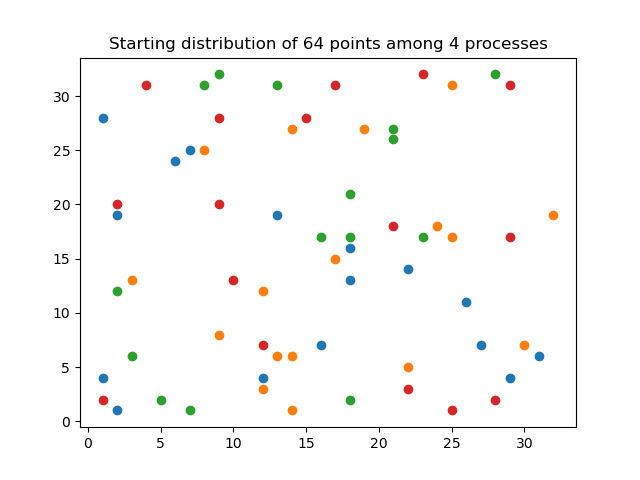
\includegraphics[width=0.45\textwidth]{img/Starting_64.png}
            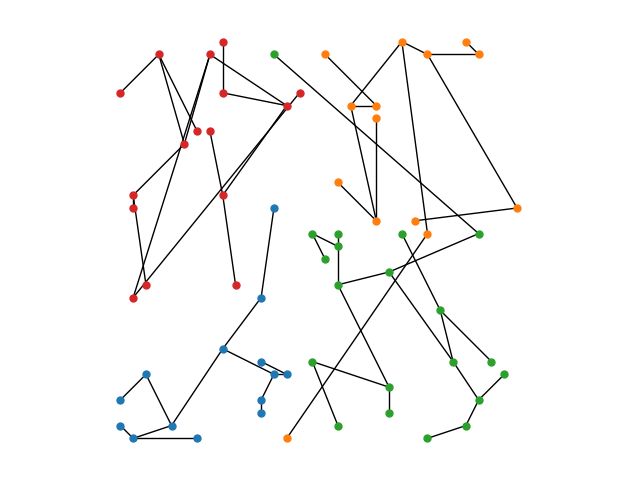
\includegraphics[width=0.45\textwidth]{img/mpistore64.png}
   %         \includegraphics[width=0.45\textwidth]{P2P_64_S.png}
    %        \includegraphics[width=0.45\textwidth]{Parallel_Kdtree_64_S.png}
     % \includegraphics[width=0.45\textwidth]{Kdtree_64_S.png}
 \caption{\textbf{Storing} pointwise exchange algorithm. 
 The original 64 random points are shown on the Left. 
On the Right, we can see the full and final kd-tree on each process (recall that each color is associated to a different process). }
\label{P2P_S}
\end{figure}



Actually, let's see what happens if we do not store/build the tree during the parallel part of the code.
In other words, let's see what happens if in the  parallel iterations, we just find global medians, move the points accordingly and split the communicators. 
This means that, in the parallel part of the code, we just move/cluster the points. 
Then, we pass these clustered points to the serial part of the code. 
In this case, for each process, the serial part of the code  effectively builds the tree from roots to leafs.
Therefore, it will first look for the local medians according to the $x$-coordinate among the already clustered points and store the splitting point in the root. The four roots are thus in each of the four quadrants, around $x\sim 8$ (blue and red communicators) and $x\sim 24$ (green and orange communicators). And so on, until the leafs nodes.
\begin{figure}
  \centering
        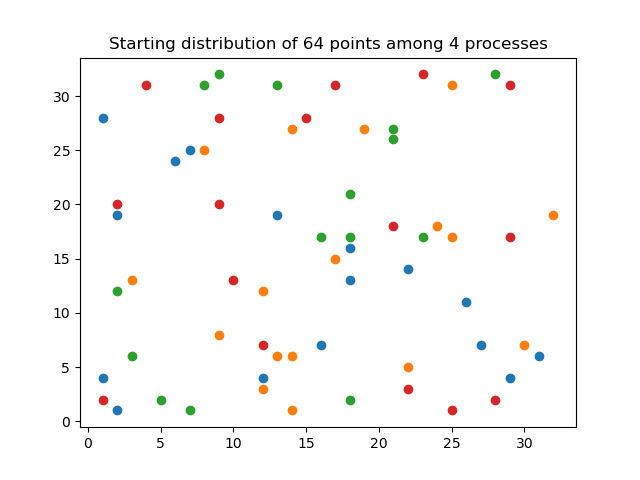
\includegraphics[width=0.45\textwidth]{img/Starting_64.png}
            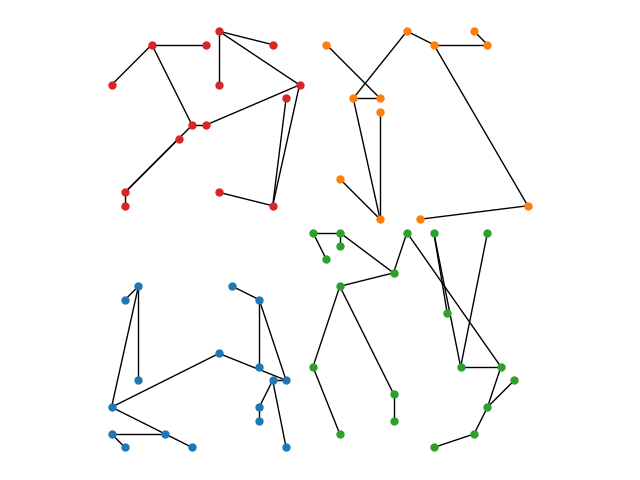
\includegraphics[width=0.45\textwidth]{img/mpiP2P.png}
%      \includegraphics[width=0.45\textwidth]{Original_64.png}
 %     \includegraphics[width=0.45\textwidth]{P2P_64_M.png}
  %    \includegraphics[width=0.45\textwidth]{Kdtree_64_M.png}
 \caption{\textbf{Moving} pointwise exchange algorithm. The original 64 random points are shown on the Left. 
On the Right, we can see the full kd-tree on each process at the end of the serial part. }
\label{P2P_M}
\end{figure}


\section{Performance model and scaling}
To test our codes we have performed strong scalability and weak scalability tests.

In the strong scalability test we have fixed the number of points to $N=10^6$ and measured the time it takes for the $\textsc{DistributedKdTreeP2P}$ function (for the MPI code) and $\textsc{SharedKdTree}$  function (for the OpenMP code) to build the kd-tree as a function of the processes $P$ with $P=1,2,4,8,16$ on a single GPU node on ORFEO cluster with two sockets of 12 cores (24 cores per node in total) $\text{Intel(R) Xeon(R) Gold 6226 CPU @ 2.70GHz}$  \footnote{Actually, hyper-threading is switched on: 2 threads per physical core} and 
\begin{itemize}
\item L1d cache:            32K
\item L1i cache:             32K
\item L2 cache:              1024K
\item L3 cache:              19712K
\end{itemize}
We compiled the code with gnu-9.3.0 compiler and openmpi-4.1.1 libraries, with $-O3$ and $-march=native$ options, using double precision numbers ($-DDOUBLE\_PRECISION$ option), generating $N$ random doubles with $drand48()$ function.
\\
The \textbf{Move} and the \textbf{Store} algorithm are pretty similar in terms of performance. We present here just the \textbf{Move} results for simplicity. 
\paragraph*{Strong scalability}
For the strong scalability test, we have compared the serial time $T(1)$ with the parallel time $T(P)$ to grow a kd-tree ($k=2$) of $N=10^6$ points to obtain the speed-up $S_p=T(1)/T(P)$. Results are shown in Table \ref{table1} and Figure \ref{Strong}.
\begin{table}[h!]
\centering
\begin{tabular}{|c|c|c|}
\hline 
P & OpenMP Time [sec] &  MPI Time [sec] \\ 
\hline 
1 & 36.8572 & 35.735761 \\ 
\hline 
2 & 21.6287  & 20.225521 \\ 
\hline 
4 & 13.3102  & 11.679689 \\ 
\hline 
8 & 9.72101 & 6.830646 \\ 
\hline 
16  & 7.26727 & 3.889892 \\ 
\hline 
\end{tabular} 
\caption{Timings for strong scalability test}
\label{table1}
\end{table}

\begin{figure}
  \centering
      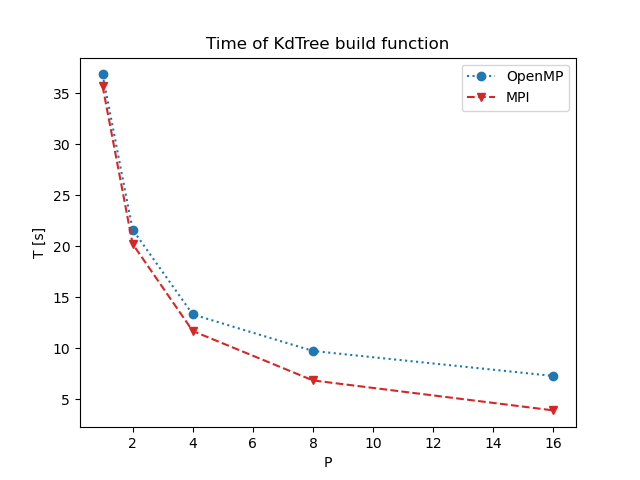
\includegraphics[width=0.45\textwidth]{img/Strong_time.png}
      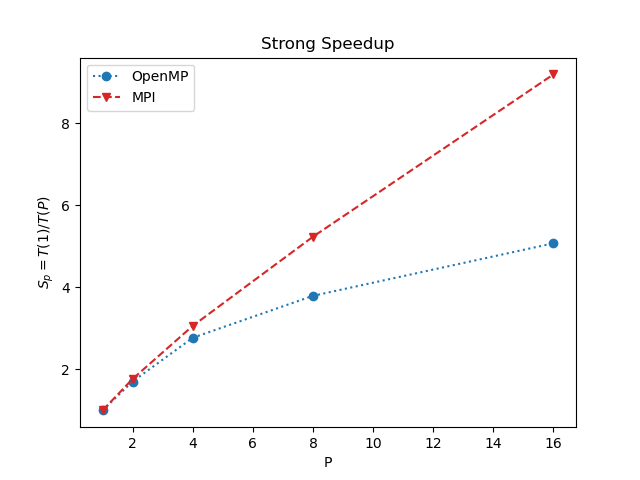
\includegraphics[width=0.45\textwidth]{img/Strong_speedup.png}
 \caption{Strong scalability: Time of building a tree of $10^6$ points as a function of $P$ with relative strong sppedup}
\label{Strong}
\end{figure}

We can see that, for small number of processes, OpenMP and MPI behave similarly, however as $P$ increases MPI performs better. Strong scaling is modeled by Amdahl's law, which arguably implies that the parallel fraction of the MPI code is larger than the OpenMP one. A possible reason for this is associated to the fact that, in the MPI code, each process proceeds in a fully parallel way on $N/P$ data (actually parallelization is only limited by communication time).
On the other hand, in the OpenMP case the $\textsc{Quickselect}$ is performed serially for the first iterations on $\mathcal{O}( N)$ points.  More specifically, one of the threads singularly $\textsc{Quickselect}$  the median among $N$ points and sorts the first $N/2$ points, then creates two tasks that are assigned to the first two available threads, and so on.
\\
Another issue is communication: while for MPI we know that communication happens when we need to find the global median and  when we pointwise exchange the points with $\textsf{MPI\_Ssend}$ and $\textsf{MPI\_Recv}$,  in the case of OpenMP we have a more obscure  hidden tasking orchestrations resulting in some overhead.\\
\paragraph*{Weak scalability}
Concerning the weak scalability,  both the number of processors and the problem size are increased, keeping the workload per processor constant.
Particularly, we have considered $N=P\times 10^6$ number of points and measured the time $T_N(P)$ it takes  to build the tree of $N$ points as a function of $P$. 
In Table \ref{table2} we report the timings  and in Figure \ref{Weak}  we have plotted the time in seconds (Left) and the weak scalability efficiency (Right) defined as $E_w=T_1(1)/T_N(P)$ as a function of $P$. 

\begin{table}[h!]
\centering
\begin{tabular}{|c|c|c|}
\hline 
P & OpenMP Time [sec] &  MPI Time [sec] \\ 
\hline 
1 & 36.5936 & 35.882094 \\ 
\hline 
2 & 44.6332 & 41.431630 \\ 
\hline 
4 & 58.5614 & 49.488500 \\ 
\hline 
8 & 78.8836& 58.178536 \\ 
\hline 
16  & 118.857 & 67.924564 \\ 
\hline 
\end{tabular} 
\caption{Timings for weak scalability test}
\label{table2}
\end{table}


\begin{figure}
  \centering
      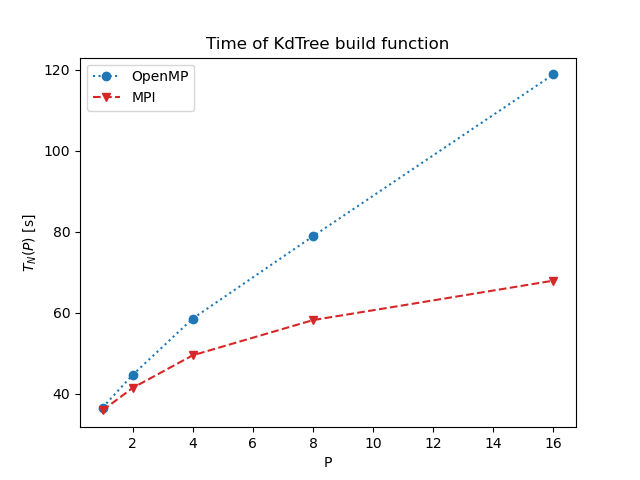
\includegraphics[width=0.45\textwidth]{img/Weak_time.png}
      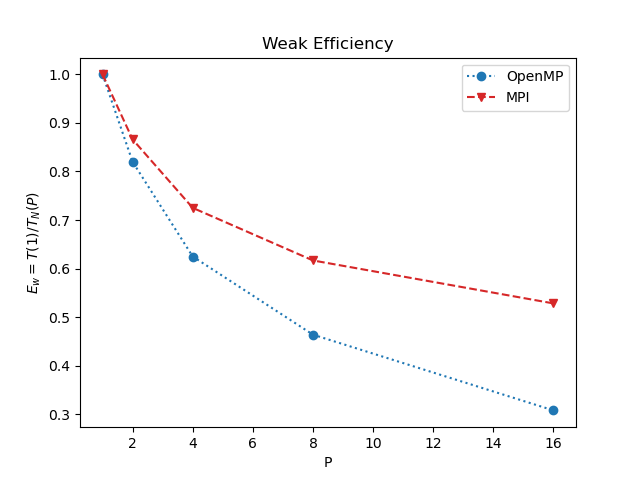
\includegraphics[width=0.45\textwidth]{img/Weak_speedup.png}
 \caption{Weak scalability: Time of building a tree of $P\times 10^6$ points as a function of $P$ with relative weak  efficiency}
\label{Weak}
\end{figure}
The result is that the MPI implementation scales better as the size of the problem is increased.

\section{Discussion}

As a conclusion, let us  summarize our results and identify possible improvements.
\\
For the assignment we implemented two codes to build a kd-tree in parallel, using two different strategies:
\begin{itemize}
\item Shared-memory kd-tree for the OpenMP code. 
\item Distributed memory kd-tree for the MPI code.
\end{itemize}
Regarding the OpenMP code, our implementation is quite straightforwardly  based on the serial code and  this might be  the  reason of lower efficiency compared to the MPI code. For instance, the serial code might not be properly optimized as we may pre-store the nodes in a contiguous memory location, instead of malloc each new node.
\\
Concerning the MPI code,  many strategies  have been considered, inspired by  \cite{xiao2016parallel}.
\\
In the end, the final/production/benchmark MPI code is based on what we called Pointwise exchange (or P2P) algorithm, declined in two possible versions \textbf{S:Store} / \textbf{M:Move} with similar performances (the only difference being in the role of the parallel part which may be relevant if one wants to implement  K-nearest neighbors algorithms). 
\\
We are aware that our implementations are not the best possible ones. Some possible way to improve our codes are:
\begin{itemize}
\item Regarding the MPI Pointwise exchange implementation, generalize the code to work with an arbitrary number of processes. Eventually, implement a re-balancing  function that keeps the number of points for process constant.
 \item Concerning the OpenMP implementation, parallelization happens only by means of creating tasks for  the left and right sub-tree. Other parts of the code might be subject to parallelization, e.g. the finding the median and dividing the points in left and right points (maybe re-organizing the code and using routines such as $\textsf{\#pragma omp parallel for}$). In general, we would like to improve performances bridging the gap with the MPI code.
 \item  Finally,  we haven't combined MPI/OpenMP. This can be done for example by calling $\textsc{SharedKdTree}$ instead of the $\textsc{SerialKdTree}$ when $|C_{\mathcal{T}}|==1$ at the end of the parallel part of the MPI code.
 This might speed up performances when  many nodes are involved, as intra-node communications are slower than inter-node ones.
\end{itemize}

\begin{thebibliography}{9}


\bibitem{xiao2016parallel}
Xiao, Bo and Biros, George (2016).
\textit{Parallel algorithms for nearest neighbor search problems in high dimensions.} SIAM Journal on Scientific Computing, 38, 5

\end{thebibliography}

\end{document}
